\section{Resultate}
Bei den Resultaten handelt es sich um die Datenstrukturen, welche in Kapitel \ref{sec:implementation} beschreiben sind.
Bei Erweiterung ``\_impr'' handelt es sich um eine Verbesserte Version wie in Kapitel \ref{subsec:impr} beschrieben.
Bei Datenstrukturen mit der Erweiterung ``\_mem'' ist ein Memorymanagement implementiert (siehe \ref{sec:mem}).
Alle Benchmarks wurden auf den TU Nebula Maschine ausgeführt. Aufgrund der beschränkten Rechenzeit auf dieser Maschine,
wurden die Test nur 10 Mal wiederholt. Die folgenden Abbildungen zeigen jeweils den Mittelwert aller Wiederholungen.
Dabei ist Anzumerken, das die Anzahl der Threads und die Anzahl der verwendeten Cores bei allen Tests identisch ist. 

\subsection{Laufzeit mit 64 Cores}

\subsubsection{Schreibvorgang}
\begin{figure}[ht!]
	\centering
	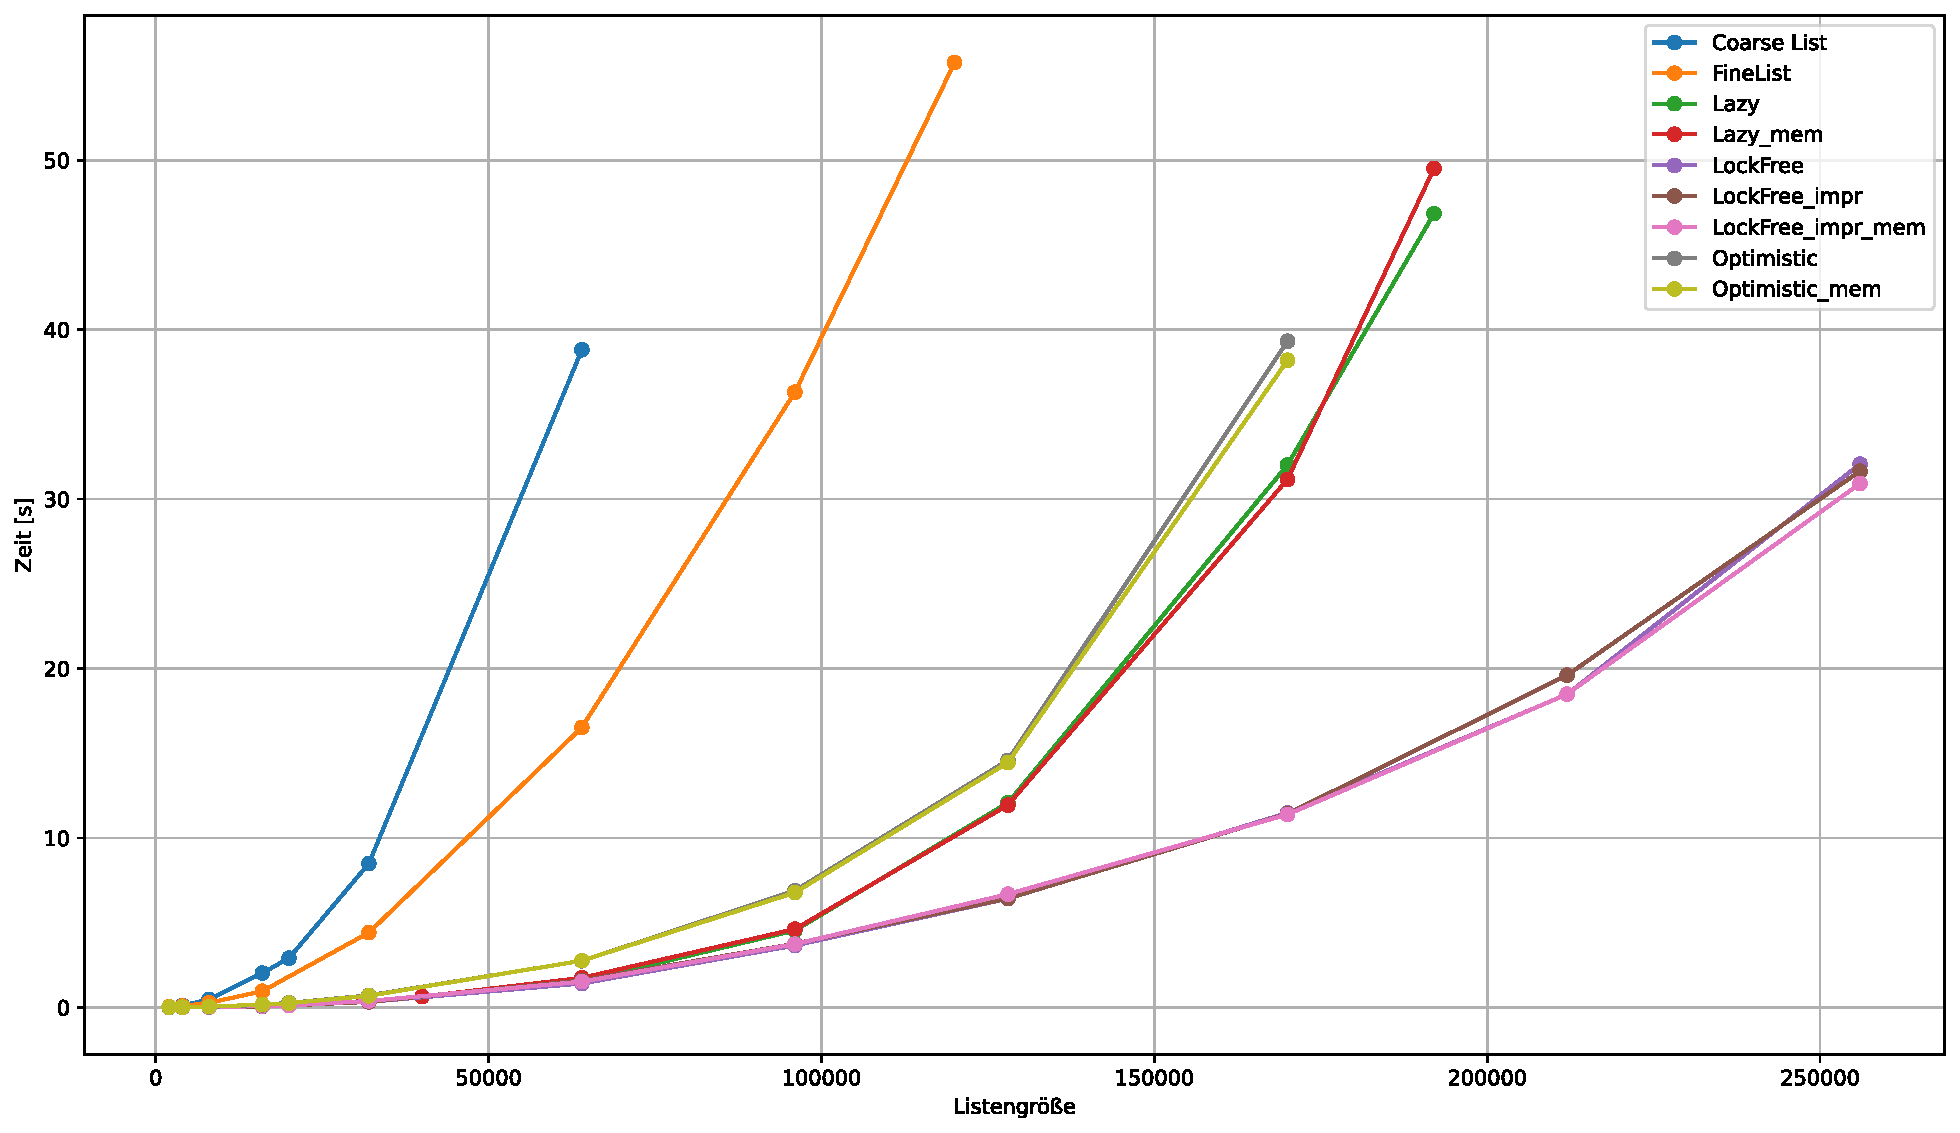
\includegraphics[width=1.0\linewidth]{./plots_pdf/write_time} 
	\caption{Laufzeit des Schreibvorganges}
	\label{fig:write_time} 
\end{figure}
Die Abbildung \ref{fig:write_time} zeigt die benötigte Laufzeit in Sekunden für das Einfügen von Elementen in eine leere Liste.
Dabei ist auf der X-Achse die Anzahl der eingefügten Elemente zu sehen. 
Das \textit{List-based set with coarse-grained locks} ist dabei am Langsamsten, da nur jeweils ein Node gleichzeitig 
Zugriff auf die Liste hat. Die schnellste Datenstruktur ist die \textit{lock-free improved with memorymanagement} Liste.

\subsubsection{Gemischter Zugriff}
\begin{figure}[ht!]
	\centering
	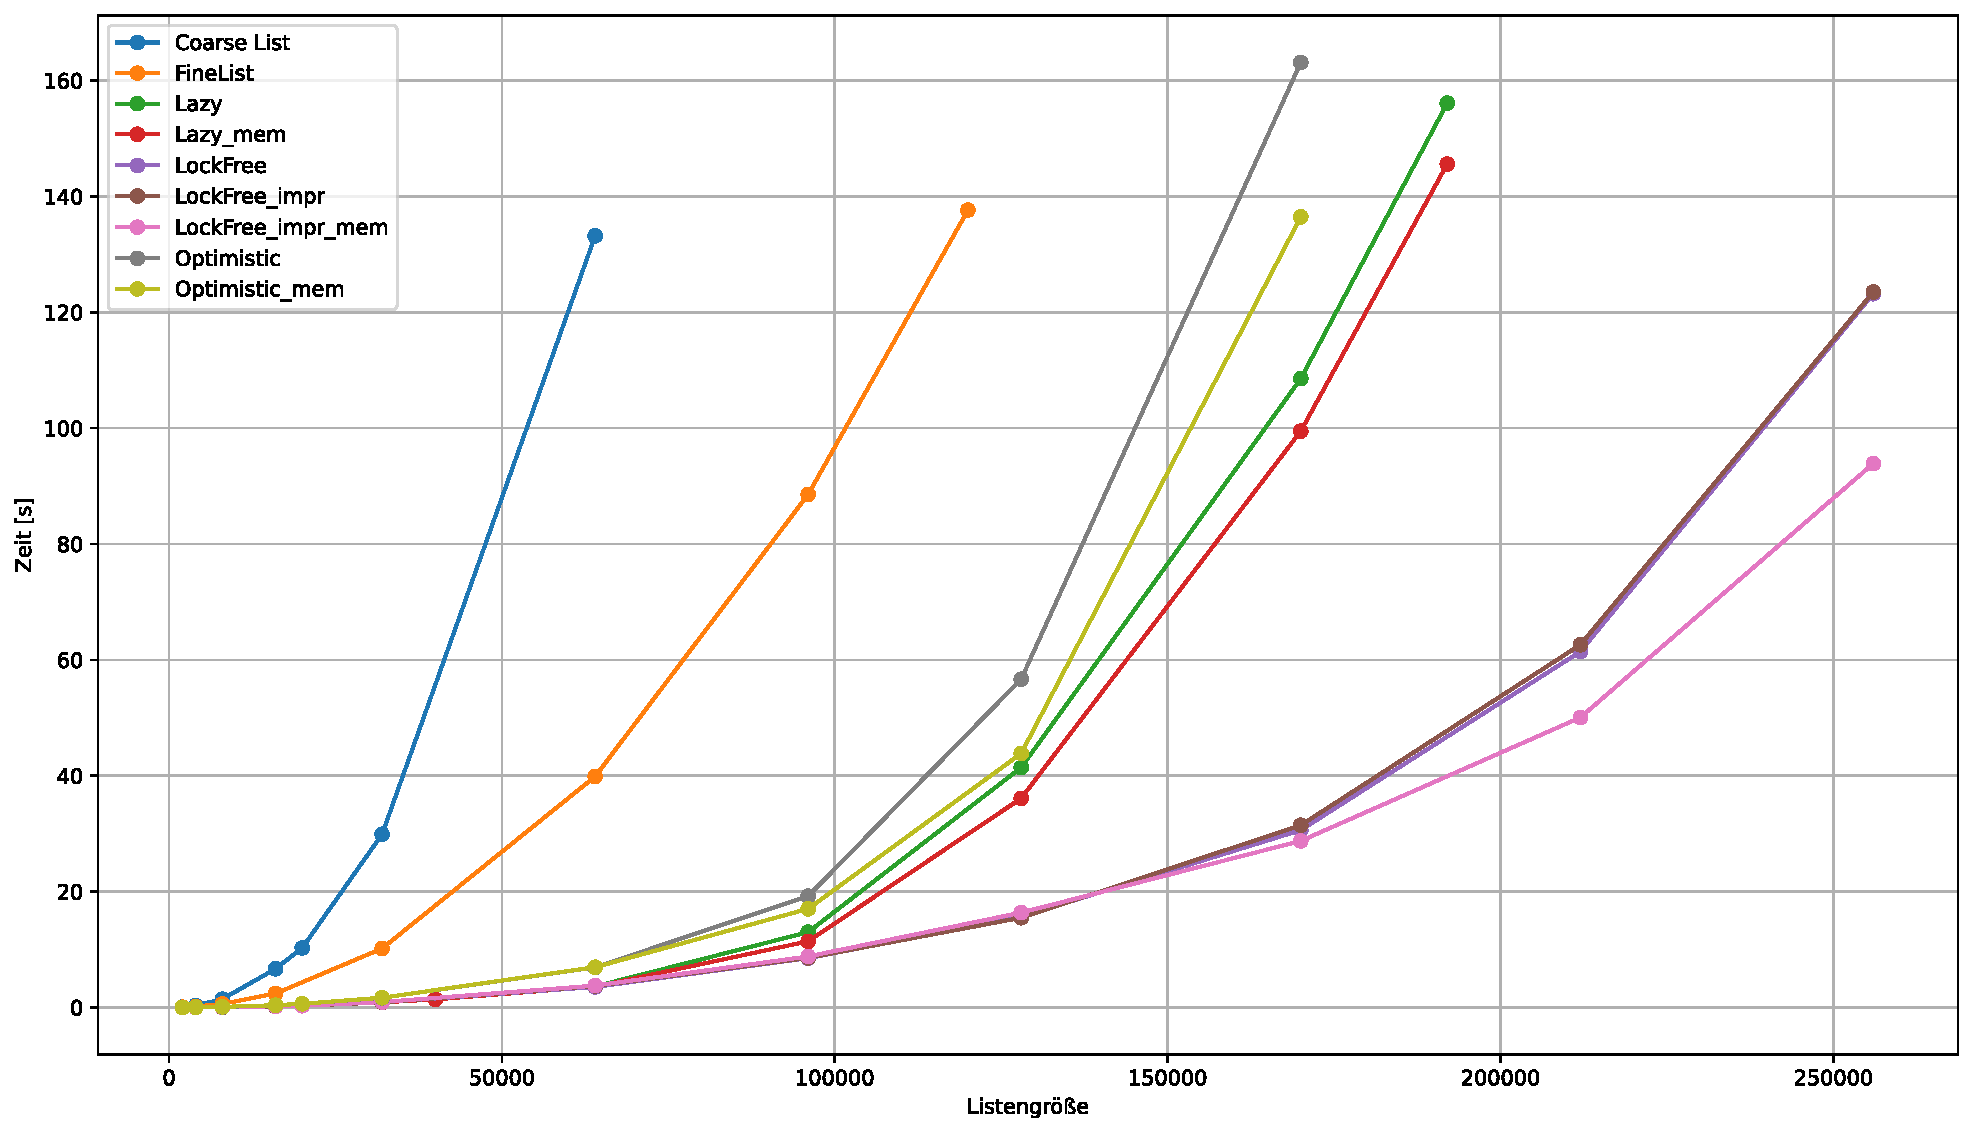
\includegraphics[width=1.0\linewidth]{./plots_pdf/mixed_time} 
	\caption{Laufzeit bei gemischten Zugriff}
	\label{fig:mixed_time} 
\end{figure}
Die Abbildung \ref{fig:write_time} zeigt die benötigte Laufzeit bei gemischten Zugriff. Dabei sind die Zugriffe folgendermaßen aufgeteilt:
 $50\%$ \textit{contain()}, $25\%$ \textit{add()} und $25\%$ \textit{remove()}.
 Dabei ist auf der X-Achse die Größe der Liste zu sehen, was auch jeweils der Anzahl der hinzugefügten und entfernten Daten entspricht. 
 Auffallend ist hier, dass Datenstrukturen mit einem implementierten Memorymanagement bei großen Listen schneller sind, obwohl
 das Memorymanagement zusätzlichen aufwand bedeutet. Eine mögliche Begründung liegt darin, dass dem Betriebssystem immer wieder 
 Speicher zurückgegeben wird und somit das auslagern von Daten aus dem Cache minimiert wird.

\subsubsection{Lesender Zugriff}
\begin{figure}[ht!]
	\centering
	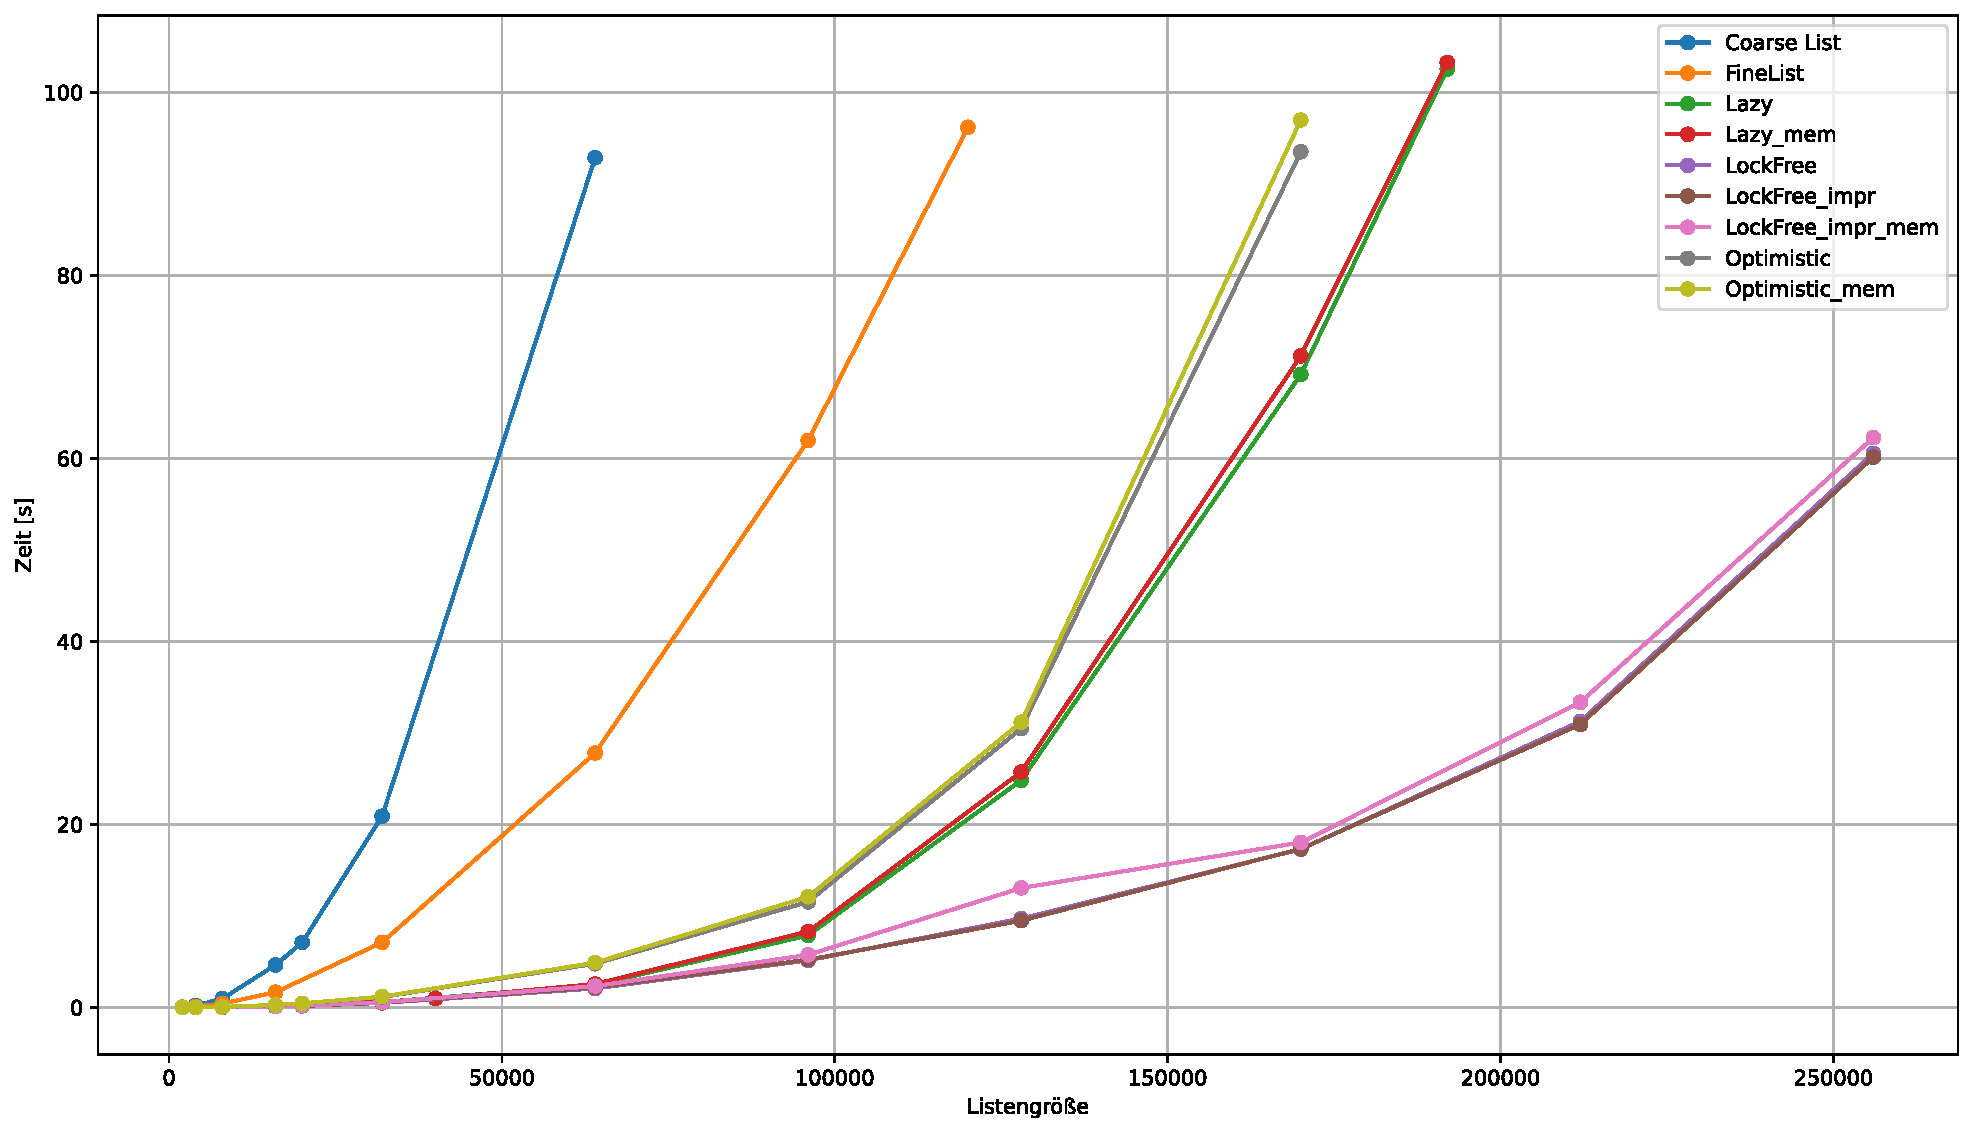
\includegraphics[width=1.0\linewidth]{./plots_pdf/check_time} 
	\caption{Laufzeit für Lesevorgang}
	\label{fig:check_time} 
\end{figure}
Die Abbildung \ref{fig:check_time} zeigt die benötigte Laufzeit, wenn auf die Datenstruktur nur mit \textit{contain()} zugegriffen wird.
Dabei wurden alle Listenelemente abgefragt. Desweiteren wurde die selbe Anzahl an Daten abgefragt, welche sich nicht in der Datenstruktur befinden.
Somit wurden doppelt so viele \textit{contain()} Anfragen ausgeführt, wie Listenelemente vorhanden sind.
Auffallend ist hier, dass beispielsweise die Lazy-Liste bei großen Listen erheblich länger benötigt, als die Lock-free list, obwohl die
\textit{contain()} Funktionen fast identisch sind. Eine mögliche Ursache ist die unterschiedliche größe der Nodes. Die Lazy-Liste beinhaltet
in ihren Nodes zusätzlich eine Variable für Mutex und einen Boolean-Variable zum markieren der gelöschten Nodes. Dieser Größenunterschied könnte für das
Memorymanagement des Betriebssystem einen erhöhten Aufwand beim laden der Nodes beim durchlaufen bedeuten. Dies ist jedoch eine Vermutung
und konnte nicht bestätigt werden.


\subsection{Neustarts von Zugriffen}
Wie bereits in Kapitel \ref{subsec:impr} beschrieben, kann es vorkommen, dass Datenstrukturen aufgrund eines konfliktes mit einem anderen
Thread einen laufenden Task neu beginnen müssen. 
In Abbildung \ref{fig:mixed_goToStart} ist zu sehen, wie oft eine laufende Funktion abgebrochen werden musste und wieder beim Listenkopf beginnen musste. 
In Abbildung \ref{fig:mixed_lostTime} ist ersichtlich, wie viel Zeit für diese Neustarts aufgewendet werden musste. \\
Bei einer Listengröße von 256 000 mit 64 Cores und 512 000 Zugriffen startet die Lock-free Liste 3163 mal neu. Dies bedeutet
einen zusätzlichen Zeitaufwand von 21 Sekunden. Somit spendet jeder Core 0,33 Sekunden mit Neustarts. Bei einer Laufzeit von 123204 Sekunden 
entspricht das 0,00028\% der Laufzeit. Da wie in Abbildung \ref{fig:mixed_lostTime} ersichtlich, steigt die zusätzliche Zeit durch Neustart erheblich.
Somit wird dies bei noch größeren Listen relevant. Im zuge dieses Projektes wurden jedoch keine größeren Listen getestet. 

\begin{figure}[ht!]
	\centering
	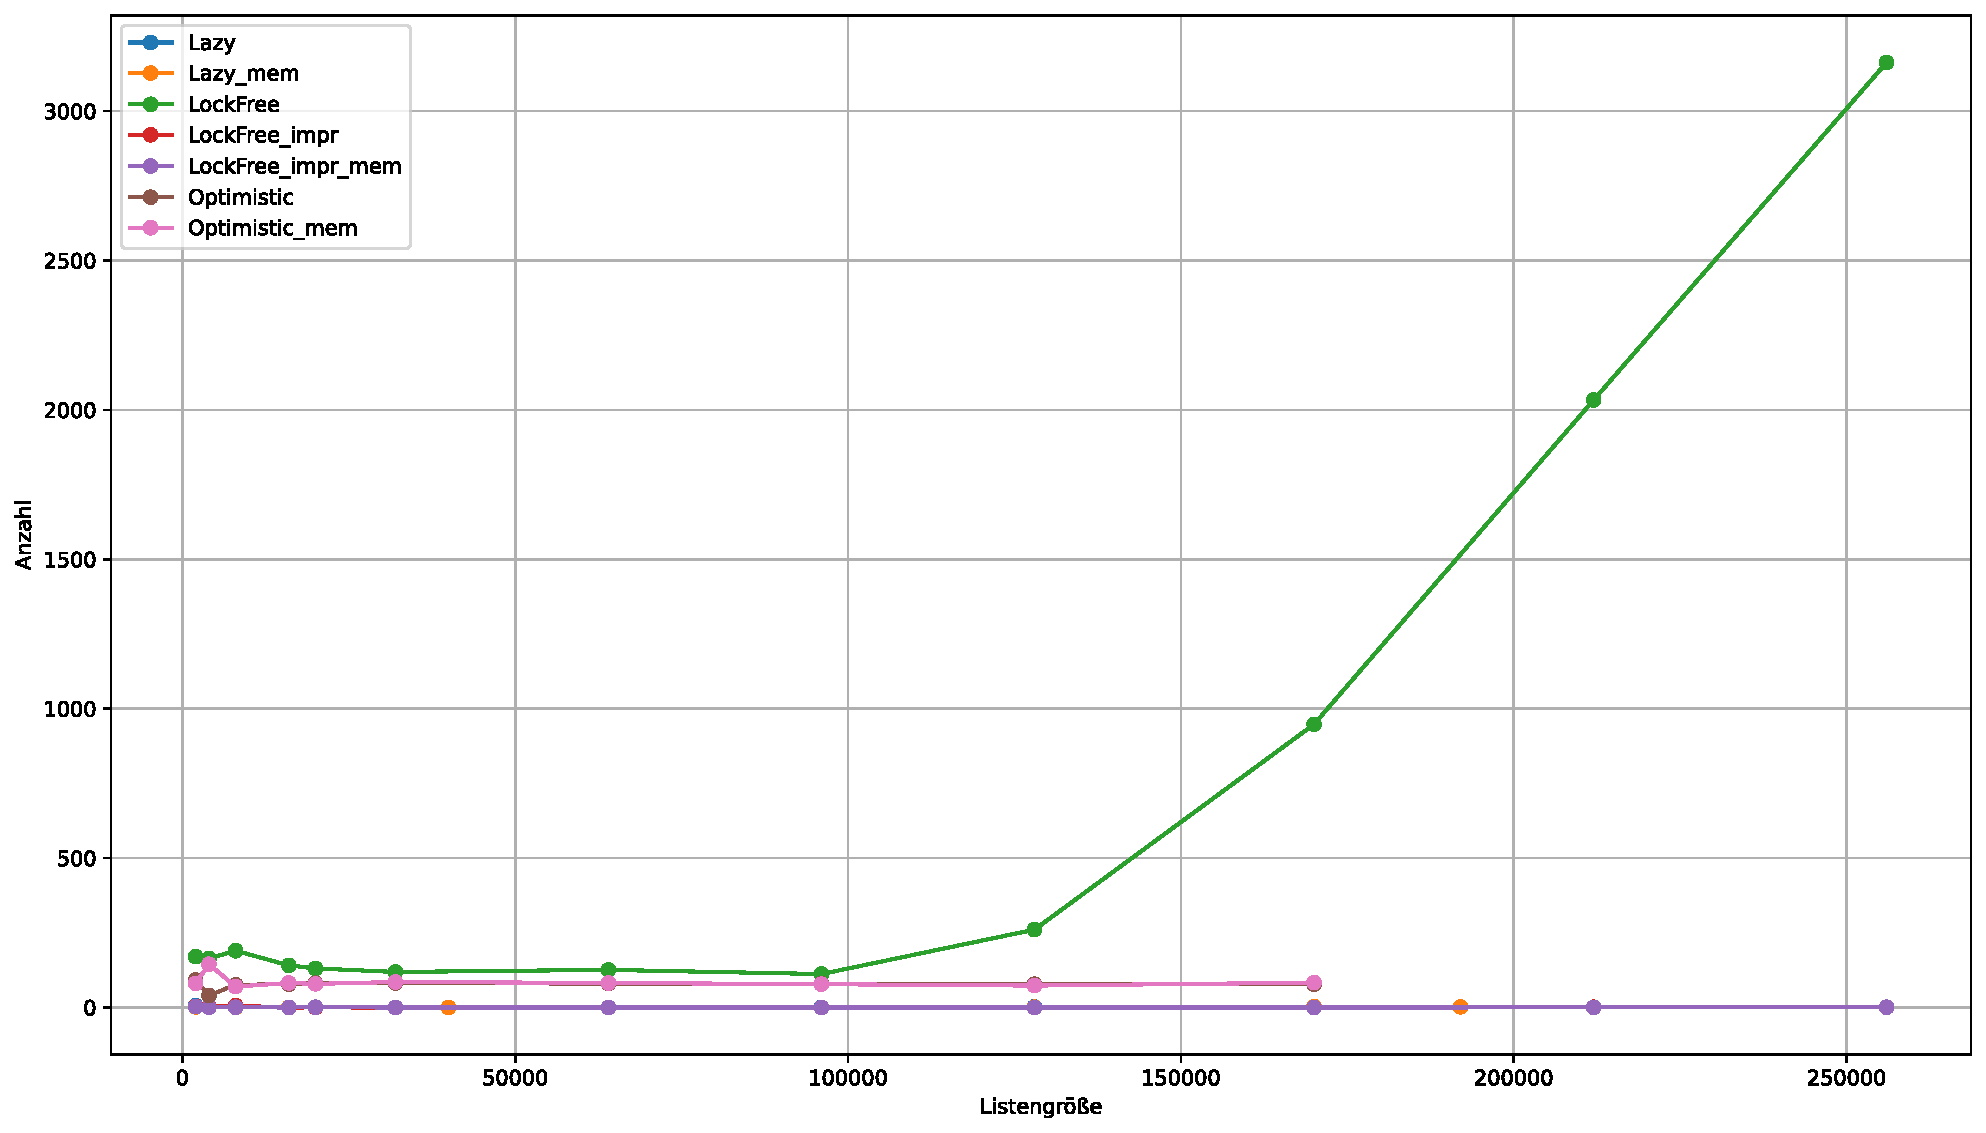
\includegraphics[width=1.0\linewidth]{./plots_pdf/mixed_goToStart.pdf} 
	\caption{Neustarts}
	\label{fig:mixed_goToStart} 
\end{figure}

\begin{figure}[ht!]
	\centering
	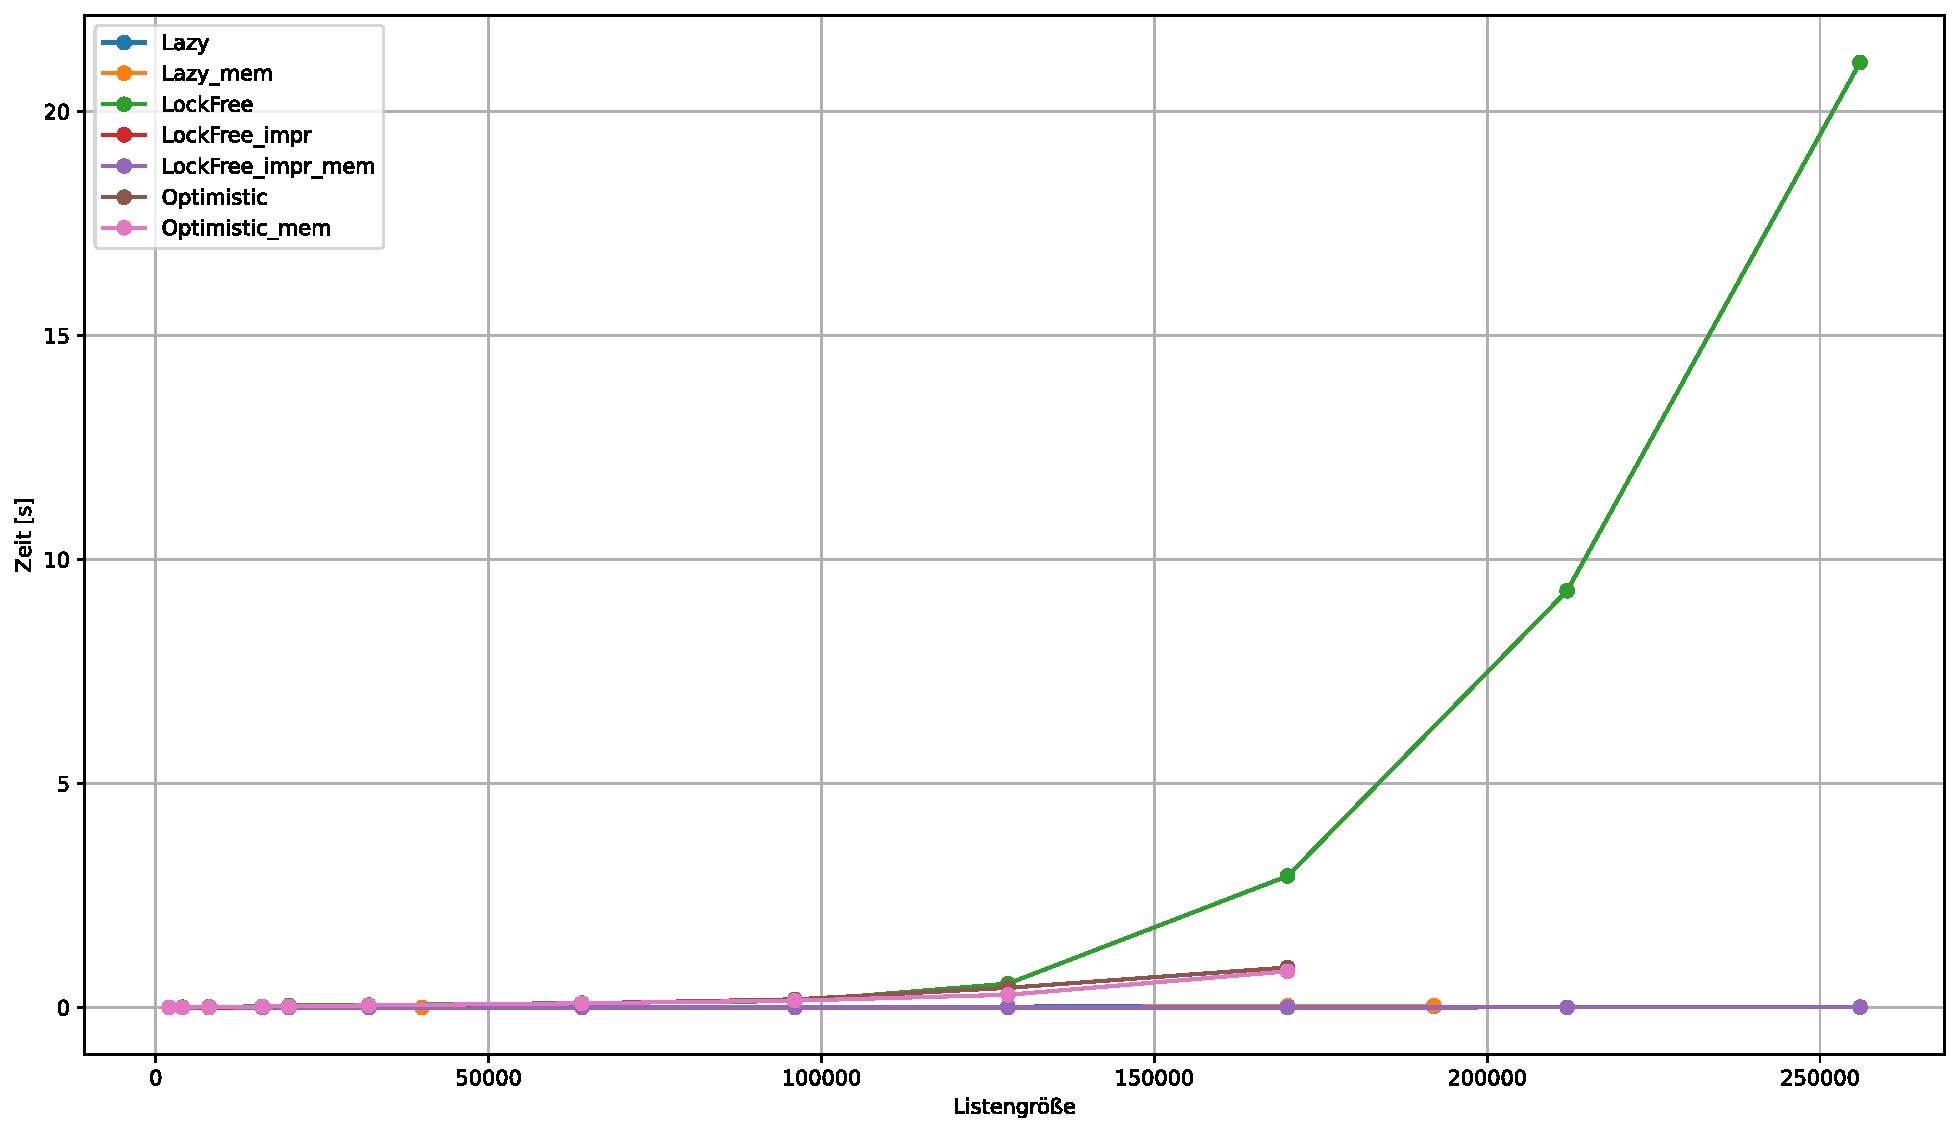
\includegraphics[width=1.0\linewidth]{./plots_pdf/mixed_lostTime.pdf} 
	\caption{Zusätzliche Zeit durch Neustarts}
	\label{fig:mixed_lostTime} 
\end{figure}


%%%%%%%%%%%%%%%%%%%%%%%%%%%%%%%%%%%%
\subsection{Laufzeit mit unterschiedlichen Cores}
\subsubsection{Vergleich 20 000 Listeneinträgen}
\label{subsec:laufzeit_20000}
Die Abbildung \ref{fig:mixed_time_cores_20000} zeigt die Laufzeit mit einer Listengröße von 20000 Einträgen bei
 \textit{contain()}, 1000 \textit{add()} und 100 \textit{remove()} zugriffen.
 Auffallend ist hier, dass
 das \textit{fine-grained locks} mit zwei Cores fast drei mal so lange benötigt als mit einem Core, da sich die einzelnen
 Threads gegenseitig behindern. 
 Weiters ist auch ersichtlich, dass bei der \textit{coarse-grained locks} Liste die Laufzeit erhöht wird, je höher
 die Anzahl der verwendeten Cores.\\
 Vergleicht man die jeweils schnellsten Datenstrukturen, kommt man auf folgende Ergebnisse:
 Ein Core mit der \textit{coarse-grained locks} Liste benötigt 4636 Sekunden und 64 Cores mit der \textit{lock-free improved with memorymanagement} Liste benötigen 311 Sekunden.
 Das entspricht einen Speedup von 14,9. \\
 Vergleicht man nun den Speedup der jeweils Schnellsten Datenstrukturen bei 20000 Listeneinträgen zwischen einem und zwei Cores mit den Speedup von 32 und 64 Cores, 
 dann erhält man folgende Ergebnisse:
 \\Seedup T1/T2=1,3 
 \\Seedup T2/T4=1,94 
 \\Seedup T8/T16=1,64 
 \\Seedup T16/T32=1,31
 \\Seedup T32/T64=1,43

 \begin{figure}[H]
	\centering
	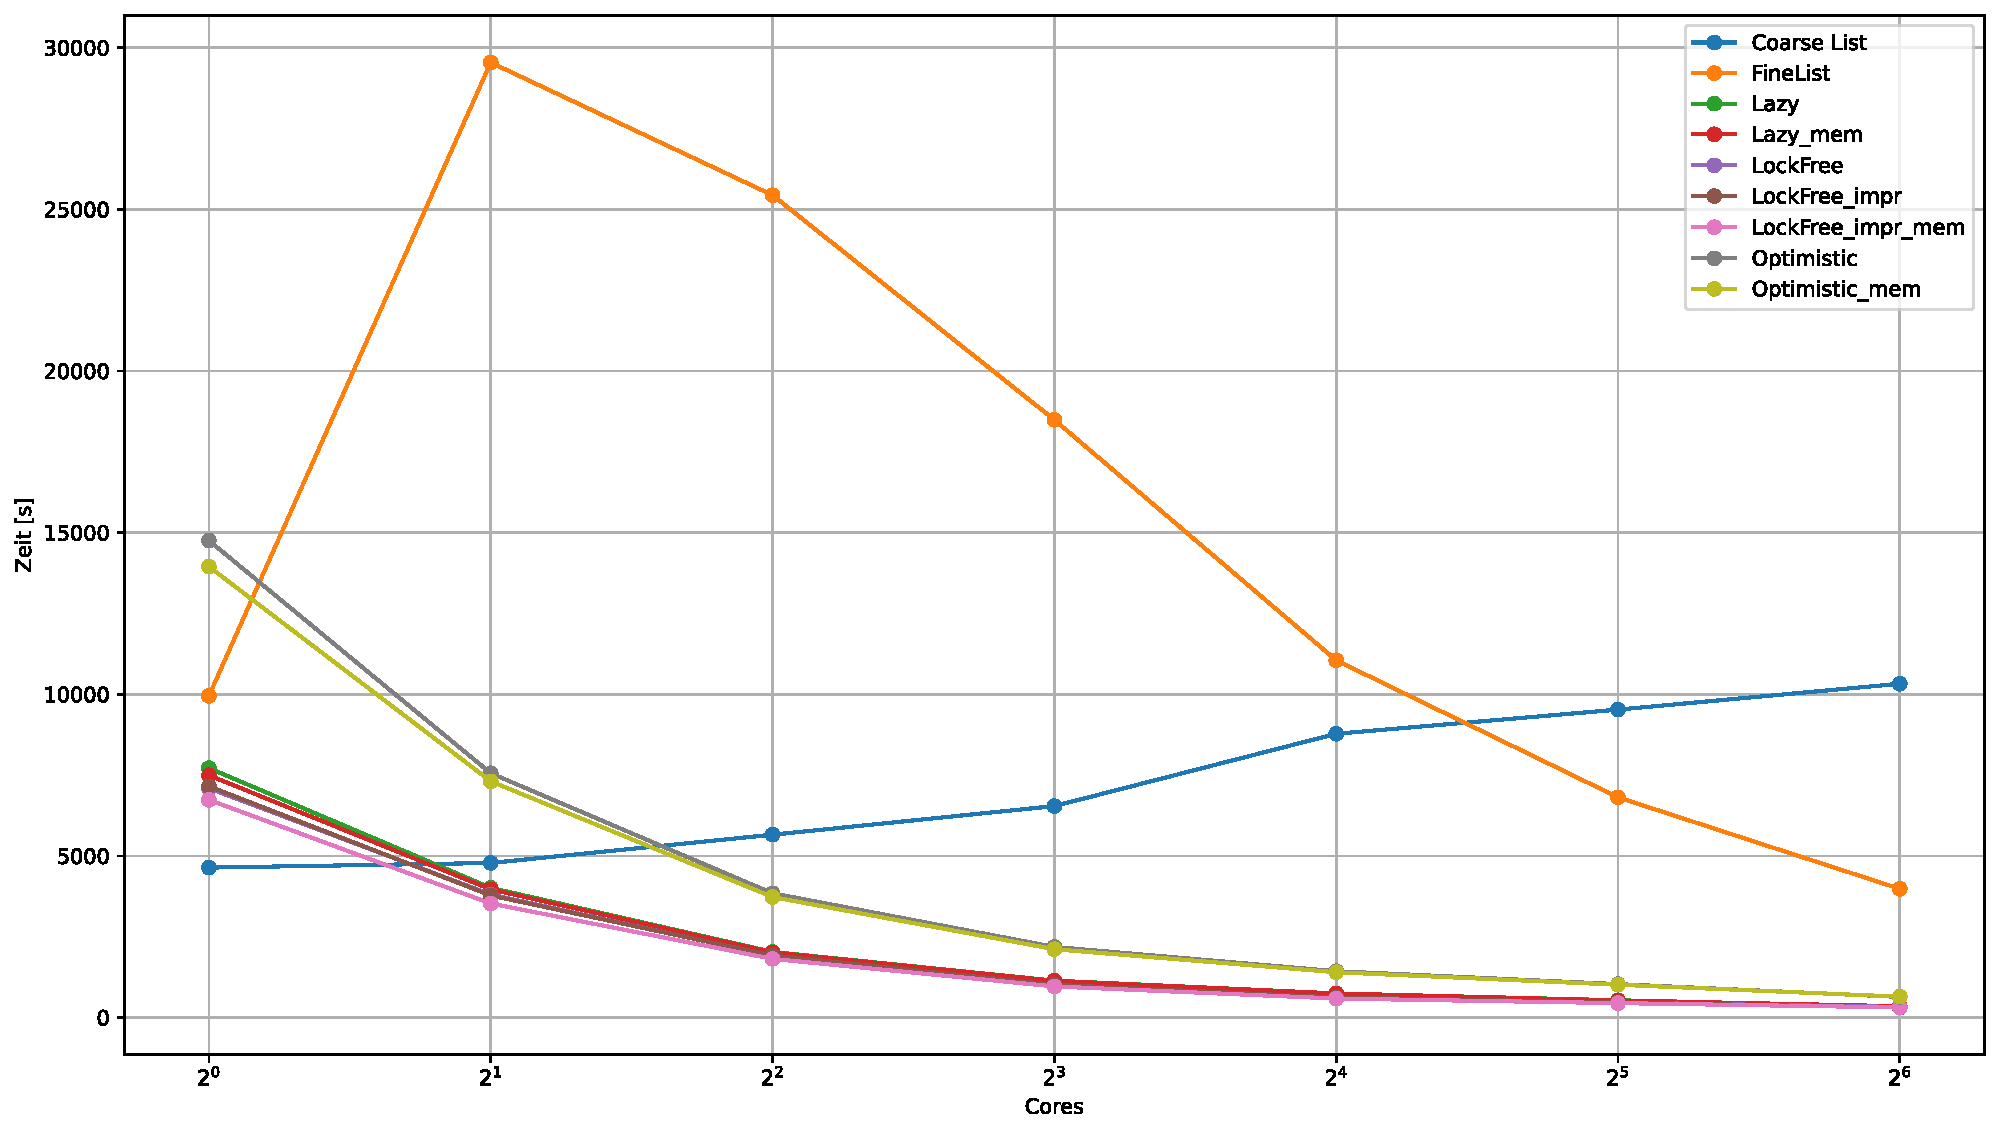
\includegraphics[width=1.0\linewidth]{./plots_pdf/mixed_time_cores_20000.pdf} 
	\caption{Laufzeit mit 20 000 Listeneinträgen} 
	\label{fig:mixed_time_cores_20000} 
\end{figure}

 \subsubsection{Vergleich 40 000 Listeneinträgen}
 \label{subsub:Vergleich_40000}
 Um die schnelleren Datenstrukturen besser zu vergleichen zu können, zeigt Abbildung \ref{fig:mixed_time_cores_40000} die Laufzeit mit verschiedenen Cores
mit der doppelten Anzahl an Listeneinträgen und zugegriffen. 
Vergleicht man nun die Speedups der schnellsten Datenstruktur (\textit{lock-free improved with memorymanagement})
mit 40 000 Einträgen, kommt man auf folgende Werte:
\\Seedup T16/T32=1,37
\\Seedup T32/T64=1,65


\begin{figure}[H]
	\centering
	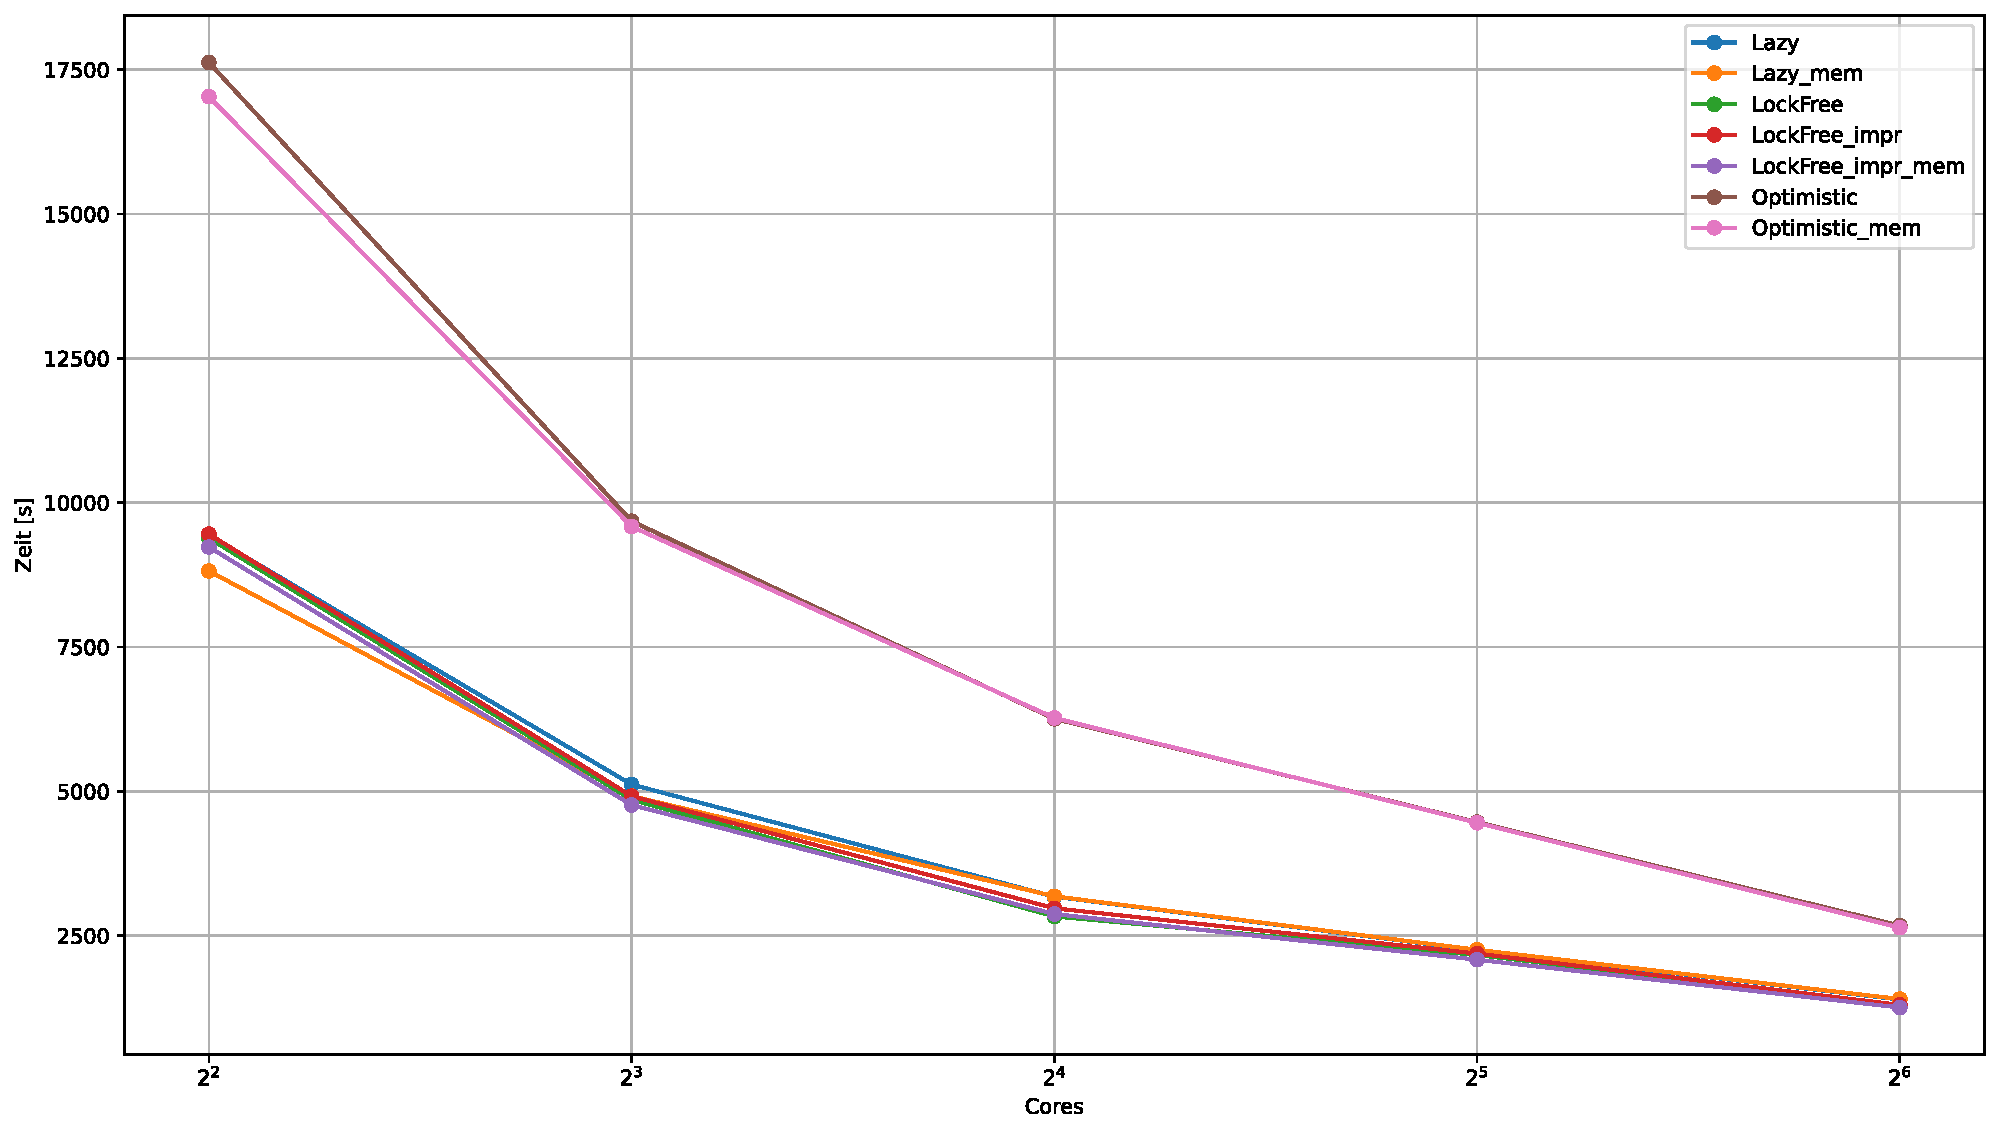
\includegraphics[width=1.0\linewidth]{./plots_pdf/mixed_time_cores_40000.pdf} 
	\caption{Laufzeit mit 40 000 Listeneinträgen}
	\label{fig:mixed_time_cores_40000} 
\end{figure}

\subsubsection{Vergleich 120 000 Listeneinträgen}
Die Abbildung \ref{fig:mixed_time_cores_120000} zeigt die Laufzeit bei
120 000 Listeneinträgen mit 240 000 zugriffen mit der gleichen Aufteilung wie die beiden vorangegangenen Abbildungen.
Vergleicht man nun die Speedups der schnellsten Datenstruktur (\textit{lock-free improved with memorymanagement} Liste)
mit 120000 Einträgen, kommt man auf folgende Werte:
\\Seedup T16/T32=1.42
\\Seedup T32/T64=1,7
\\ Vergleicht man diese Werte mit den Speedups von \ref{subsec:laufzeit_20000} und \ref{subsub:Vergleich_40000}, 
ist ersichtlich, dass das vergrößern der Liste keinen signifikanten Einfluss auf den Speedup hat. 



\begin{figure}[H]
	\centering
	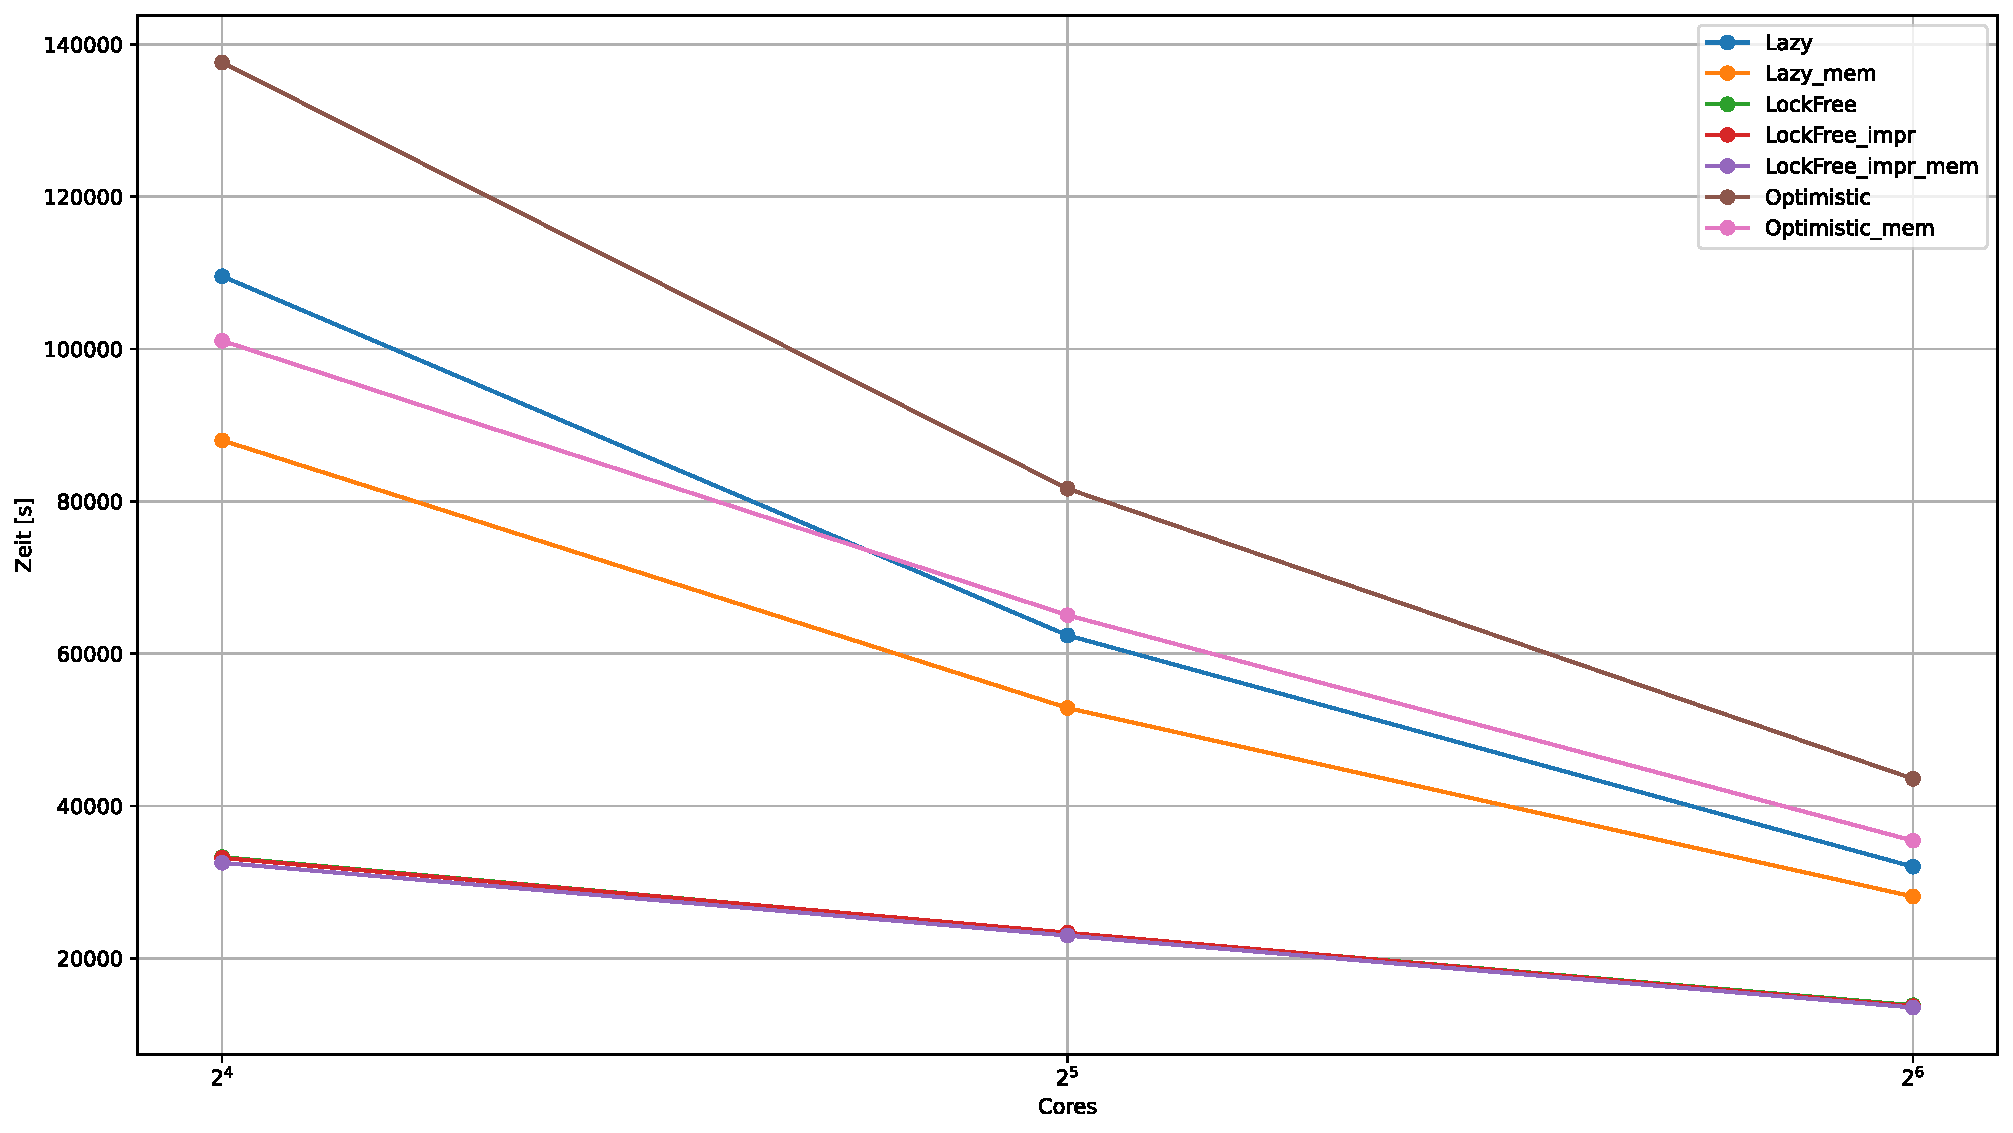
\includegraphics[width=1.0\linewidth]{./plots_pdf/mixed_time_cores_120000.pdf} 
	\caption{Laufzeit mit 120 000 Listeneinträgen}
	\label{fig:mixed_time_cores_120000} 
\end{figure}